% This file was created by matlab2tikz.
%
%The latest updates can be retrieved from
%  http://www.mathworks.com/matlabcentral/fileexchange/22022-matlab2tikz-matlab2tikz
%where you can also make suggestions and rate matlab2tikz.
%
\definecolor{mycolor1}{rgb}{0.00000,0.44700,0.74100}%
%
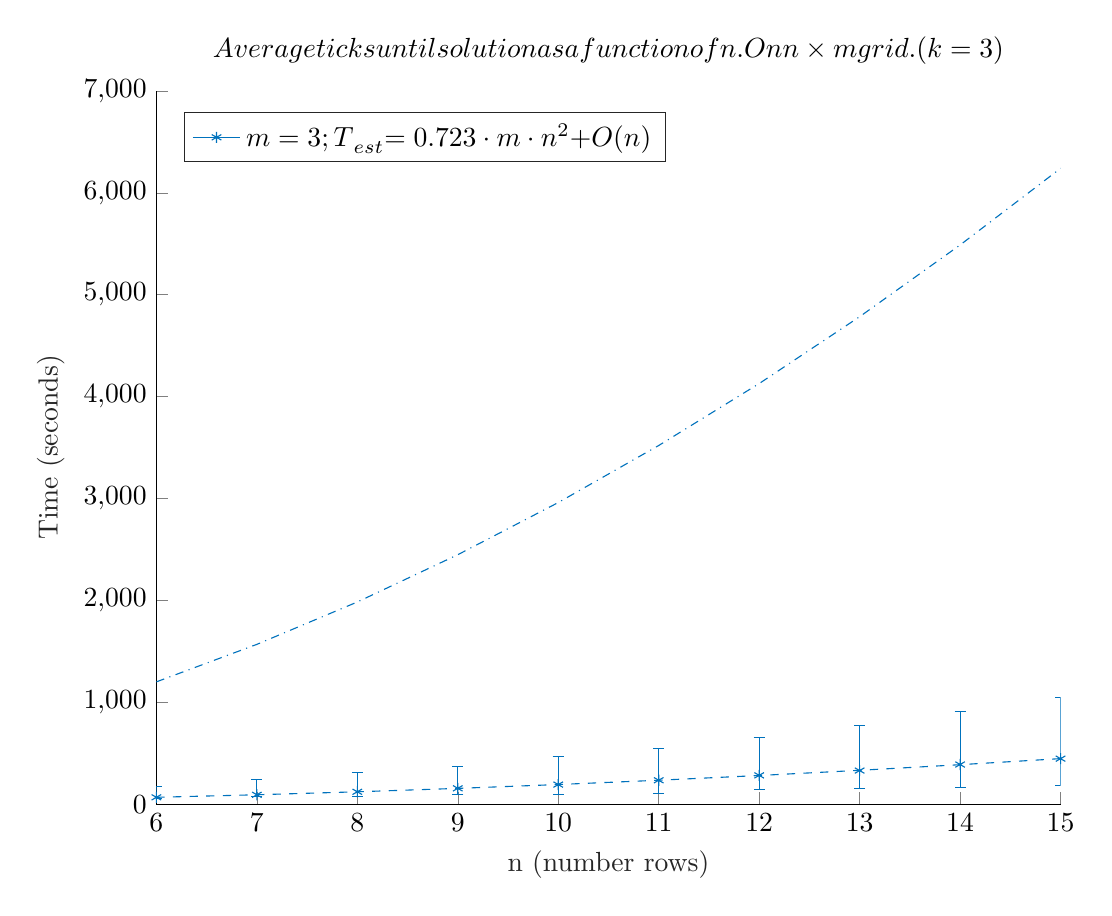
\begin{tikzpicture}

\begin{axis}[%
width=4.521in,
height=3.566in,
at={(0.758in,0.481in)},
scale only axis,
xmin=6,
xmax=15,
xlabel style={font=\color{white!15!black}},
xlabel={n (number rows)},
ymin=0,
ymax=7000,
ylabel style={font=\color{white!15!black}},
ylabel={Time (seconds)},
axis background/.style={fill=white},
title style={font=\bfseries},
title={$\text{Average ticks until solution as a function of n. On n }\times\text{ m grid. (k = 3)}$},
axis x line*=bottom,
axis y line*=left,
legend style={at={(0.03,0.97)}, anchor=north west, legend cell align=left, align=left, draw=white!15!black}
]
\addplot [color=mycolor1, draw=none, mark=asterisk, mark options={solid, mycolor1}]
  table[row sep=crcr]{%
6	66.874\\
7	91.86\\
8	121.156\\
9	155.144\\
10	191.816\\
11	234.246\\
12	282.3\\
13	329.44\\
14	388.884\\
15	446.218\\
};
\addlegendentry{$\text{m = 3; T}_{\text{est}}\text{ = 0.723}\cdot\text{m}\cdot\text{n}^\text{2}\text{ + O(n)}$}

\addplot [color=mycolor1, dashdotted, forget plot]
  table[row sep=crcr]{%
6	1200\\
7	1568\\
8	1984\\
9	2448\\
10	2960\\
11	3520\\
12	4128\\
13	4784\\
14	5488\\
15	6240\\
};
\addplot [color=mycolor1, draw=none, forget plot]
 plot [error bars/.cd, y dir = both, y explicit]
 table[row sep=crcr, y error plus index=2, y error minus index=3]{%
6	66.874	108	8\\
7	91.86	148	14\\
8	121.156	192	44\\
9	155.144	216	64\\
10	191.816	276	98\\
11	234.246	316	128\\
12	282.3	376	141\\
13	329.44	440	174\\
14	388.884	520	225\\
15	446.218	600	262\\
};
\addplot [color=mycolor1, dashed, forget plot]
  table[row sep=crcr]{%
6	67.053563636361\\
7	91.8672727272717\\
8	121.020860606061\\
9	154.514327272728\\
10	192.347672727274\\
11	234.520896969698\\
12	281.034000000001\\
13	331.886981818182\\
14	387.079842424242\\
15	446.61258181818\\
};
\end{axis}
\end{tikzpicture}%